\section{Dataset real}
\label{sec:datasetReal}
Debido a que las animaciones encontradas en el banco de animaciones no eran las suficientes y estaban descompensadas se decidió crear una herramienta para poder recoger los datos de usuarios.

\subsection{Funcionamiento de la herramienta}
La herramienta se conecta con el traje de captura de movimiento mediante una malla proporcioanda por el plugin (TO DO: REFERENCIA A LA WEB DEL PLUGIN).
Este plugin se conecta a la aplicación mediante la dirección IP de la máquina que ejecuta Axis Studio y sockets TCP a un puerto que puedes configurar en la aplicación de Axis Studio. (TO DO: PONER CAPTURA DE LA CONFIGURACIÓN DE AXIS STUDIO)

Una vez conectado se le debe pasar al componente MocapDumper el nombre de la animación que se va a grabar, el número de toma de esa animación y un número que sirva como identifidor de usuario.
Finalmente cuando la herramienta está ejecutándose y se le da a la tecla ''espacio'' genera un CSV del formato ''animación\_User\_Número de ususario\_Take\_Número de toma'' (si el fichero ya existía lo sobreescribe), escribe la misma cabecera del CSV que se menciona en el apartado anterior (TO DO: HACER TABLA Y REFERENCIARLA) y pone la aplicación en estado de grabación.
En este estado la aplicación escribe en cada frame todos los componentes de la posición y rotación (en forma de vector de ángulos de Euler) de cada hueso.
Cuando se le vuelve a dar al espacio la aplicación cierra el fichero y vuelve a un estado de no grabación.

En la figura \ref{fig:MocapDumper} se muestra un diagrama de cómo se conectan los diferentes componentes necesarios en esta herramienta

\begin{figure}[H]
	\centering
	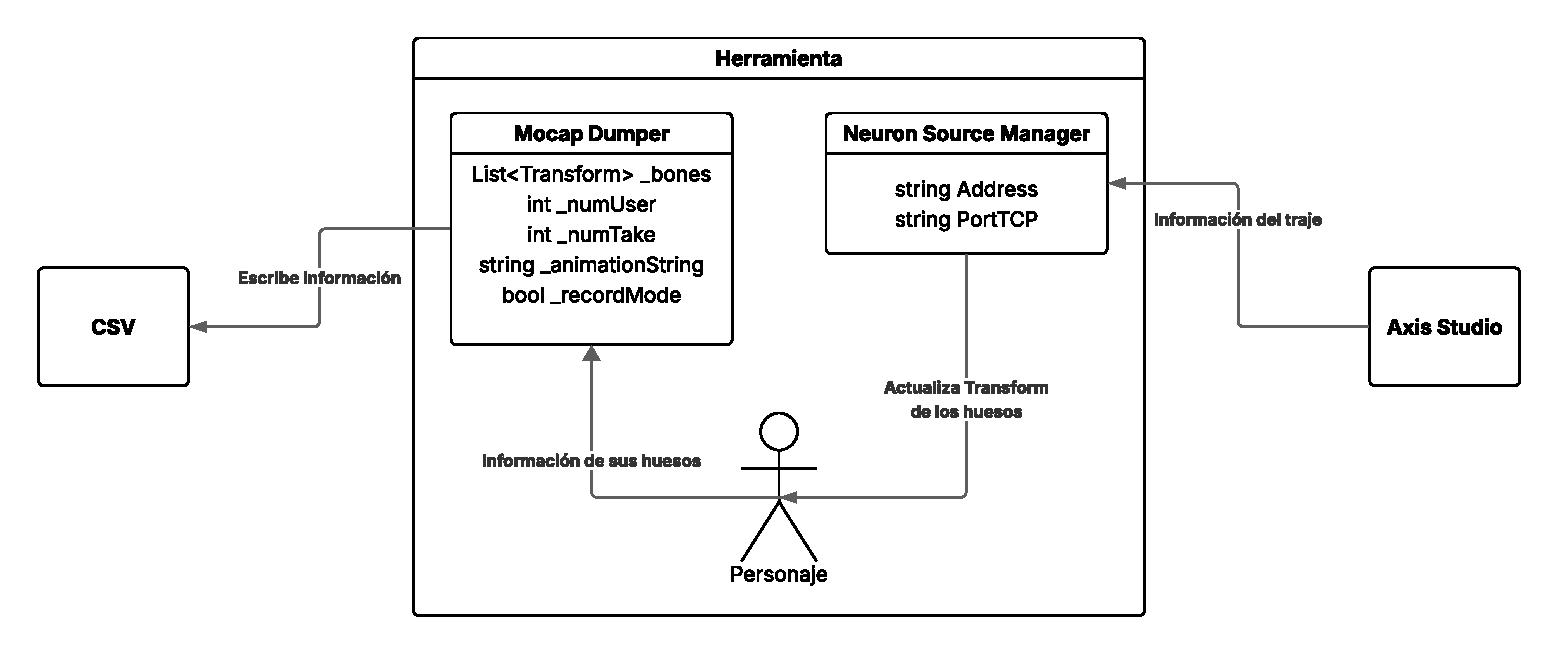
\includegraphics[width=1\textwidth]{Imagenes/Vectorial/MocapDumper.pdf}
	\caption{Diagrama de la conexión entre los distintos componentes de la herramienta, llamada Mocap Dumper}
	\label{fig:MocapDumper}
\end{figure}

\subsection{Recogida de datos}
La recogida de datos consistió en ponerle el traje de captura de movimiento a los usuarios y pedirles que realizasen tres tomas de cada uno de los gestos, a excepción del gesto de baile, ya que de ese gesto había basantes más datos que el resto.

Para ello se creó un formulario para que los usuarios interesados en ello se apuntasen. En el formulario se explicaba el objetivo de la prueba y se numeraban los datos que iban a ser pedidos en la prueba. Los campos a rellenar eran: 

\begin{enumerate}
	%\renewcommand{\theenumi}{\alph{enumi}}
	\item Correo
	\item Aceptar recogida de datos
	\item Posible hueco en un horario, en huecos de una hora de lunes a viernes y de 9:00 a 20:00
\end{enumerate}

Una vez creado el formulario se creó un cartel (TO DO: PONER FOTO DEL CARTEL) el cual se colgó en redes y se colgó en distintas facultades (NO SÉ SI PROCEDE COMENTARLO PERO BUENO), teniendo como resultado que se apuntasen 75 personas en el formulario.

Lo siguiente era tener un sitio en el que hacer las pruebas. Debido a que las pruebas requerían movimiento era preciso un lugar en el que los usuarios se pudiesen mover sin dificultades y que no estuviese a la vista para preservar la intimidad de los mismos.

TO DO: HABLAR DE LA RAMIFICACIÓN Y PODA HECHA PARA CONSEGUIR LOS HUECOS

Finalmente desde el día 14/04/2025 a las 9:00 hasta el día 17/04/2025 a las 19:30 se pudo grabar en el despacho 216 (Sala de grabaciones) de la Facultad de Informática de la Universidad Complutense de Madrid.
De los 75 usuarios apuntados finalmente se presentaron 65, consiguiendo así 975 animaciones en formato CSV, 195 de cada gesto. (TO DO: PONER FOTOS DE LAS PRUEBAS Y LOS USUARIOS)

TO DO: HABLAR DE LOS DATOS PEDIDOS DE LOS USUARIOS Y SUS RESULTADOS, SUS ESTADÍSTICAS Y TODO ESO

TO DO: HABLAR DE LAS ANIMACIONES YA PROCESADAS EN QUÉ SE QUEDA Y DAR PASO A LA PARTE DE LOS MODELOS

Una vez recogidos y procesados los datos recogidos en las pruebas de usuario se procede al entrenamiento de los distintos modelos para su posterior comparativa.